\subsection{Assembly task} % (fold)
\label{sub:assembly_task}

There are four different types of components, numbered $1$ through
$4$, which can be combined to form larger components according to
the assembly plans in Fig. \ref{fig:assembly_plans}.  Components
bond together through bi-directional connections at sites along
their perimeters. The last step in each plan is the production of a
final assembly, $F1$ or $F2$.  The assembly task is executed by a
group of robots in an arena that is sufficiently large to ignore the
dynamics of small-scale interactions, shown in Fig.
\ref{fig:overall_arena}. Initially, many copies of components of
type $1$ through $4$ are randomly scattered. throughout the arena.
There are exactly as many of these components as are needed to
create a specified number of final assemblies, and the number of
robots equals the total number of scattered components. Each robot
knows the assembly plans a-priori and has the ability to recognize
component types, pick up a component, combine it with one that is
being carried by another robot, and disassemble a component it is
carrying.

Our objective is to define robot controllers for moving around the
arena and for picking up, assembling, and disassembling components
so that the robots produce target numbers of final assemblies as
quickly as possible.

%, that can be combined into two possible final assemblies, $F1$ and
%$F2$.  Each final assembly is built from components $1, 3, 4$, and
%two copies of $2$ according to the plans in Fig.
%\ref{fig:assembly_plans}.

    \begin{figure}[h!]
        \centering
            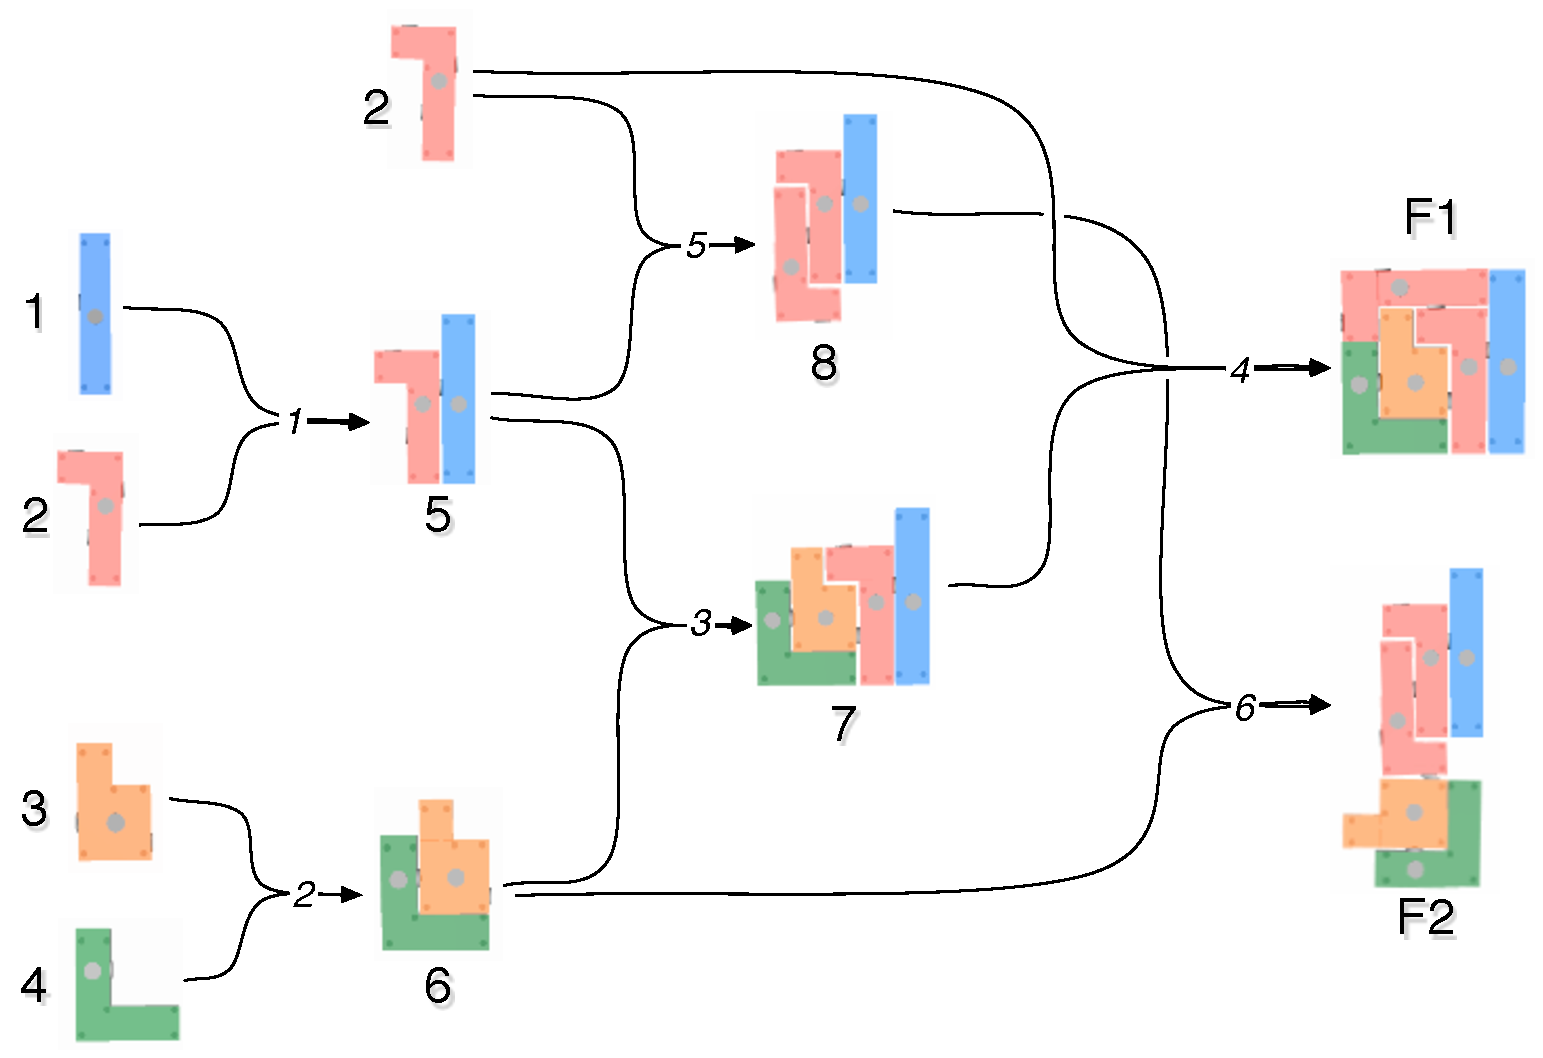
\includegraphics[width=8cm]{img/assembly_plans.pdf}
        \caption{Assembly plans for final assemblies F1 and F2.}
        \label{fig:assembly_plans}
    \end{figure}

    \begin{figure}[h]
        \centering
            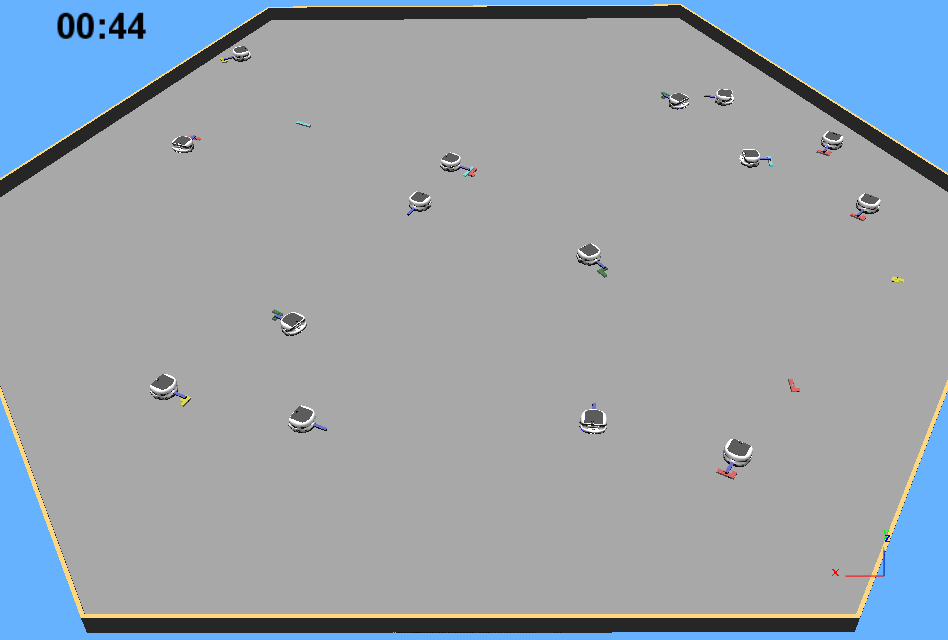
\includegraphics[width=8cm]{img/overall_arena_3.png}
        \caption{Snapshot of the arena in the realistic physical simulation.
Robots carry components at the end of a protruding arm. The
connector at the tip of this arm can rotate freely to align
components for assembly.}
        \label{fig:overall_arena}
    \end{figure}

% subsection assembly_task (end)

\subsection{Microscopic model} % (fold)
\label{sub:stochastic_assembly}
    We study a control policy for the robot taking inspiration of chemical processes:
    random movement patterns with probabilistic assembly upon encountering, as well as
    random disassemblies.

    Our models assume a well-mixed characteristic of the system, as it is the case in
    most chemical processes. Thus our robots moves according to a random walk, which we
    verify to satisfy this property.
    Robots communicate with each others and with pieces using local range radio (60cm).
    When they encounter a lying piece, they carry it and start looking for another robot
    with a compatible piece, according to the assembly plans. When a compatible encounter
    takes place, the robots align their pieces and assemble them. One robot carry the newly
    build mid-assembly while the other other resumes looking for another lying piece. When
    disassembling, one part of the mid-assembly is dropped on the floor and has to be found
     again by another robot.

    We keep track of the populations of pieces and assemblies, for several experiments with
    random initial positions of pieces and robots in the arena.

    In order to control the assembly policies, we can modify directly the rates of assemblies
     and disassemblies. More precisely, we control the probabilities of starting an assembly
     or a disassembly.

    This simulation is done in a realistic physics simulator, Webots \cite{Michel:2004p10762}.
     It gives us a precise microscopic discrete model of the assembly task.
% subsection stochastic_assembly (end)

Various methods exist to numerically simulate the evolution of a
system governed by this model
\cite{Gillespie:2007p1788,Puchalka:2004p4312}.
